\documentclass[a4paper]{scrartcl}
\usepackage[cm]{fullpage}
\usepackage{amsmath, amssymb, esint}
\usepackage{siunitx}

\usepackage{tikz, pgfplots}
\pgfplotsset{
    compat = 1.12,
    plot-scatter/.style = {
        only marks,
        error bars/.cd,
        x dir = both, y dir = both,
        x explicit, y explicit
    }
}

\DeclareSIUnit\litre{\liter}

\begin{document}

\title{PHYS3113: Stirling Engine}
\author{ \\ \\ }
\date{2017-05-09}
\maketitle

\begin{abstract}
    A ``real'' two arm Stirling engine was tested with a \(\Delta T\) ranging from \SI{135 \pm 1}{\kelvin} to \SI{197 \pm 1}{\kelvin} and angular frequencies \(f\) ranging from \SI{375 \pm 10}{\per\minute} to \SI{855 \pm 10}{\per\minute} to examine its torque, work and power output capabilities, and how they varied against angular frequency.
\end{abstract}

\section{Materials and Methods}
Please refer to the operating instructions of the experiment and the prework.

For part 2, instead of taking the reading from the multimeter, the oscilloscope was instead used to collect time series voltage data, where its mean and standard deviation was used instead.

For part 3, the pressure and volume-proportional voltage data was collected from the oscilloscope. They were then passed through a 101-point window cubic Savitzky--Golay filter to reduce the quantisation error in the values, before being integrated to find the energy output per period. Unfortunately, this analysis doesn't produce any error value, so instead we manually estimate a \SI{5}{\percent} error from the graph alone.

\section{Results}
\subsection{Part 1: Mechanical Power}
\begin{figure}
    \centering
    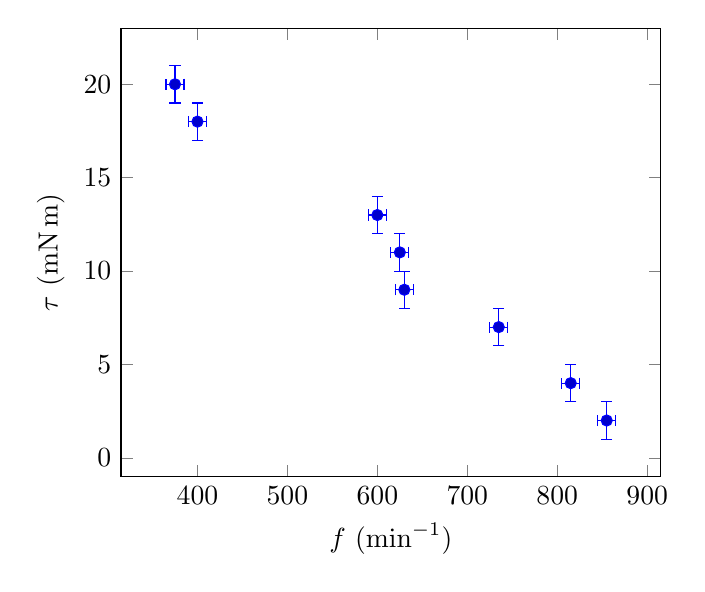
\begin{tikzpicture}
        \begin{axis}[
            xlabel = \(f\) (\si{\per\minute}),
            ylabel = \(\tau\) (\si{\milli\newton\metre})
        ]
            \addplot +[plot-scatter] table [
                x error = xerror,
                y error = yerror
            ] {
                x   y   xerror  yerror
                855 2   10      1
                815 4   10      1
                735 7   10      1
                630 9   10      1
                625 11  10      1
                600 13  10      1
                400 18  10      1
                375 20  10      1
            };
        \end{axis}
    \end{tikzpicture}
    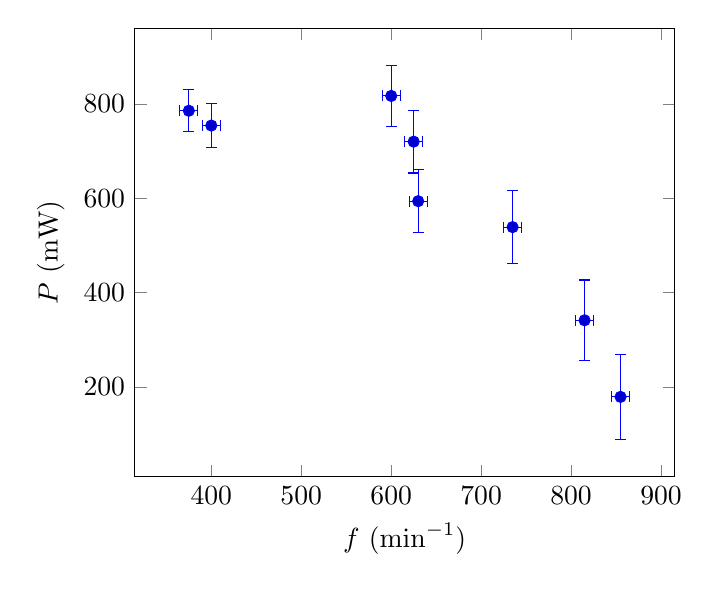
\begin{tikzpicture}
        \begin{axis}[
            xlabel = \(f\) (\si{\per\minute}),
            ylabel = \(P\) (\si{\milli\watt})
        ]
            \addplot +[plot-scatter] table [
                x error = xerror,
                y error = yerror
            ] {
                x   y       xerror  yerror
                855 179.1   10      89.6
                815 341.4   10      85.4
                735 538.8   10      77.3
                630 593.8   10      66.6
                625 719.9   10      66.5
                600 816.8   10      64.3
                400 754.0   10      45.9
                375 785.4   10      44.5
            };
        \end{axis}
    \end{tikzpicture}
    \caption{Torque as measured by the torque meter against the angular frequency at the time, as well as the computed power. \(\Delta T\) increased as \(\tau\) increased, from \SI{135 \pm 1}{\kelvin} to \SI{197 \pm 1}{\kelvin}}
    \label{fig:part1}
\end{figure}

Figure \ref{fig:part1} contains the important data recorded for this part of the experiment. One can see a clear, approximately linear negative slope in the torque graph. The power graph has a flat top of sorts, before falling towards zero too.

Unfortunately during the period of the measurements, the \(\Delta T\) value varied significantly, though approximately proportional to the torque value. This means that the slope of the torque graph is steeper than what it would actually be for a constant \(\Delta T\).

Higher torques could not be measured with our apparatus, since they stalled the engine. This indicates the largest torque value we obtained was near the maximum torque of the engine.

\subsection{Part 2: Electrical Generator}
\begin{figure}
    \centering
    \begin{tikzpicture}
        \begin{axis}[
            xlabel = \(f\) (\si{\per\minute}),
            ylabel = \(P\) (\si{\milli\watt})
        ]
            \addplot +[plot-scatter] table [
                x error = xerror,
                y error = yerror
            ] {
                x   y       xerror  yerror
                660 0       10      0
                %445 1.047   10      0.291 % ΔT = 120
                %540 17.961  10      4.743 % ΔT = 126
                %440 76.893  10      27.987 % ΔT = 118
                665 2.407   10      0.591
                560 19.267  10      4.953
                600 39.776  10      10.994
                545 100.14  10      41.246
                520 132.34  10      60.424
            };
        \end{axis}
    \end{tikzpicture}
    \begin{tikzpicture}
        \begin{axis}[
            xlabel = \(f\) (\si{\per\minute}),
            ylabel = \(W_T\) (\si{\milli\joule})
        ]
            \addplot +[plot-scatter] table [
                x error = xerror,
                y error = yerror
            ] {
                x   y       xerror  yerror
                660 0       10      0
                665 0.217   10      0.053
                560 2.064   10      0.532
                600 3.978   10      1.101 
                545 11.025  10      4.545
                520 15.27   10      6.978
            };
        \end{axis}
    \end{tikzpicture}
    \caption{Power output of the electrical generator against the angular frequency at the time, as well as the computed work per cycle. \(\Delta T = \SI{150 \pm 10}{\kelvin}\)}
    \label{fig:part2}
\end{figure}

Figure \ref{fig:part2} contains the important data recorded for this part of the experiment. We can see an approximate negative slope on both the power and work-per-cycle graphs.

Fortunately the \(\Delta T\) for this experiment was relatively constant at \SI{150 \pm 10}{\kelvin}, though we still obtained some data points that had significant variance due to some low resistance settings of the shunt resistor.

Higher loads could not be measured because they stalled the engine. This indicates the largest power output we obtained was near the maximum of the engine.

\subsection{Part 3: PV Diagram}
\begin{figure}
    \centering
    \begin{tikzpicture}
        \begin{axis}[
            xlabel = \(f\) (\si{\per\minute}),
            ylabel = \(W_T\) (\si{\milli\joule})
        ]
            \addplot +[plot-scatter] table [
                x error = xerror,
                y error = yerror
            ] {
                x   y       xerror  yerror
                %880 214.6   10      10.7 % ΔT = 107
                570 260.6   10      13.0
                540 257.2   10      12.9
                435 259.6   10      13.0
                500 263.6   10      13.2
            };
        \end{axis}
    \end{tikzpicture}
    \begin{tikzpicture}
        \begin{axis}[
            xlabel = \(f\) (\si{\per\minute}),
            ylabel = \(P\) (\si{\watt})
        ]
            \addplot +[plot-scatter] table [
                x error = xerror,
                y error = yerror
            ] {
                x   y       xerror  yerror
                570 2.476   10      0.131
                540 2.315   10      0.124
                435 1.882   10      0.104
                500 2.197   10      0.118
            };
        \end{axis}
    \end{tikzpicture}
    \caption{Work per cycle from the PV diagram under differing loads, as well as computed power. \(\Delta T = \SI{195 \pm 5}{\kelvin}\)}
    \label{fig:part3}
\end{figure}
\begin{figure}
    \centering
    \includegraphics[height = 10cm]{part3/unloaded.png}
    \caption{Representative PV loop from the measurements. This specific loop was from the unloaded case}
    \label{fig:part3-loop}
\end{figure}

For each measurement in this part of the experiment, we obtained loops all looking quite similar to Figure \ref{fig:part3-loop}, and in fact their \(P \:\mathrm{d}V\) value was also quite similar, as can be seen in the left graph of Figure \ref{fig:part3}. This indicates that regardless of the load, each cycle of the engine produces the same amount of work.

The difference that comes in to play is when you consider the speed the engine is operating at. If the same amount of work goes out of each cycle, but you fit more cycles into per unit time, you get more power the faster the engine, as can be seen in the right graph of Figure \ref{fig:part3}.

\section{Discussion}
Our torque measurements in part 1 matches what we would expect for an engine that is near its unloaded operating speed: torque decreases until it reaches its unloaded speed. The fact that it turned out to be approximately linear is likely the result that we're only looking at a small window of its operating speeds, since in general torque-speed graphs are rarely linear.

We also get a somewhat negative slope in both power and work per cycle in part 2 and the electrical generator, which is what we still expect. Our variables has a lot more variance here, however, so further measurements should be taken to confirm this.

Finally, we get equal work per cycle no matter how loaded the engine is in part 3. This is expected, as all thermodynamic cycles' work output is independent of any speed variable. However, this does not contradict the previous two experiments of decreasing work/torque/power output with increasing speed, as increasing the speed also increases the losses (e.g., frictional, drag) experienced by the engine.

If we consider the maximum power we obtained (\SI{790 \pm 40}{\milli\watt} at a frequency of \SI{375 \pm 10}{\per\minute}) in part 1), compared to the values we obtained from part 3 (assuming constant power per cycle: \SI{1630 \pm 30}{\milli\watt}), we can see that the engine is \SI{48 \pm 3}{\percent} efficient in converting work done by the gas to mechanical work at \(f = \SI{375 \pm 10}{\per\minute}\)..

While we have obtained graphs that look close to what we expect, there is too much variation in the data for parts 1 and 2 to give an accurate conclusion to what they should actually be.

\section{Conclusion}
(\emph{From Abstract}) A ``real'' two arm Stirling engine was tested with a \(\Delta T\) ranging from \SI{135 \pm 1}{\kelvin} to \SI{197 \pm 1}{\kelvin} and angular frequencies \(f\) ranging from \SI{375 \pm 10}{\per\minute} to \SI{855 \pm 10}{\per\minute} to examine its torque, work and power output capabilities, and how they varied against angular frequency.

\end{document}